\chapter{Reference chapter} \label{section_chapter_xxx}


\section{Introduction} \label{section_chapter_xxx_lelabel}

The goal of this study is to establish how a calculation procedure can be developed
which has calculation times and costs acceptable to industrial norms so as to optimise
the design of composite pressure vessels whilst ensuring quantifiable levels of confidences
in their performance. This will be achieved by Finite Element numerical simulation.

The goal of this study is to establish how a calculation procedure can be developed
which has calculation times and costs acceptable to industrial norms so as to optimise
the design of composite pressure vessels whilst ensuring quantifiable levels of confidences
in their performance. This will be achieved by Finite Element \index{Finite Element} numerical simulation.


\section{Exemple de bibliographie} \label{section_chapter_xxx_exemple_de_biblio}

Pour un auteur Batdorf \cite{Batdorf1982a}. Pour deux auteurs Aveston and Kelly \cite{Aveston1973a}.
Pour plus de deux auteurs Aveston {\it et al.} \cite{Aveston1971a}.

\section{Exemple de tableau} \label{section_chapter_xxx_exemple_de_tableau}

Sur le tableau (Tab. \ref{table_chapter_xxx_lelabel}), on voit.
Les resultats montrent la correlation des mesures (Tab. \ref{table_chapter_xxx_lelabel}).


\begin{table}[!ht]
 \begin{center}
    \begin{tabular}{|c|c|c|c|c|c|c|}
   \hline
Cases   & $\gamma$ & $\ln K$ \\
\hline
1D-A  & -0.071 & 10.01 \\
1D-B    & -0.619 & 9.76 \\
1D-C    & -0.596 & 9.73 \\
2D-A    & -0.533 & 10.43 \\
2D-B    & -0.971 & 10.79 \\
2D-C    & -0.591 & 10.69 \\
3D      & -0.820 & 10.86 \\
   \hline
\end{tabular}
    \caption{
    \label{table_chapter_xxx_lelabel}
    Linear Fitting.
    }
 \end{center}
\end{table}


\section{Exemple de figure} \label{section_chapter_xxx_exemple_de_figure}

Sur la figure (Fig. \ref{figure_chapter_xxx_lelabel}), on voit.
Les resultats montrent la correlation des mesures (Fig. \ref{figure_chapter_xxx_lelabel}).

\begin{figure}[!ht]
	\begin{center}
		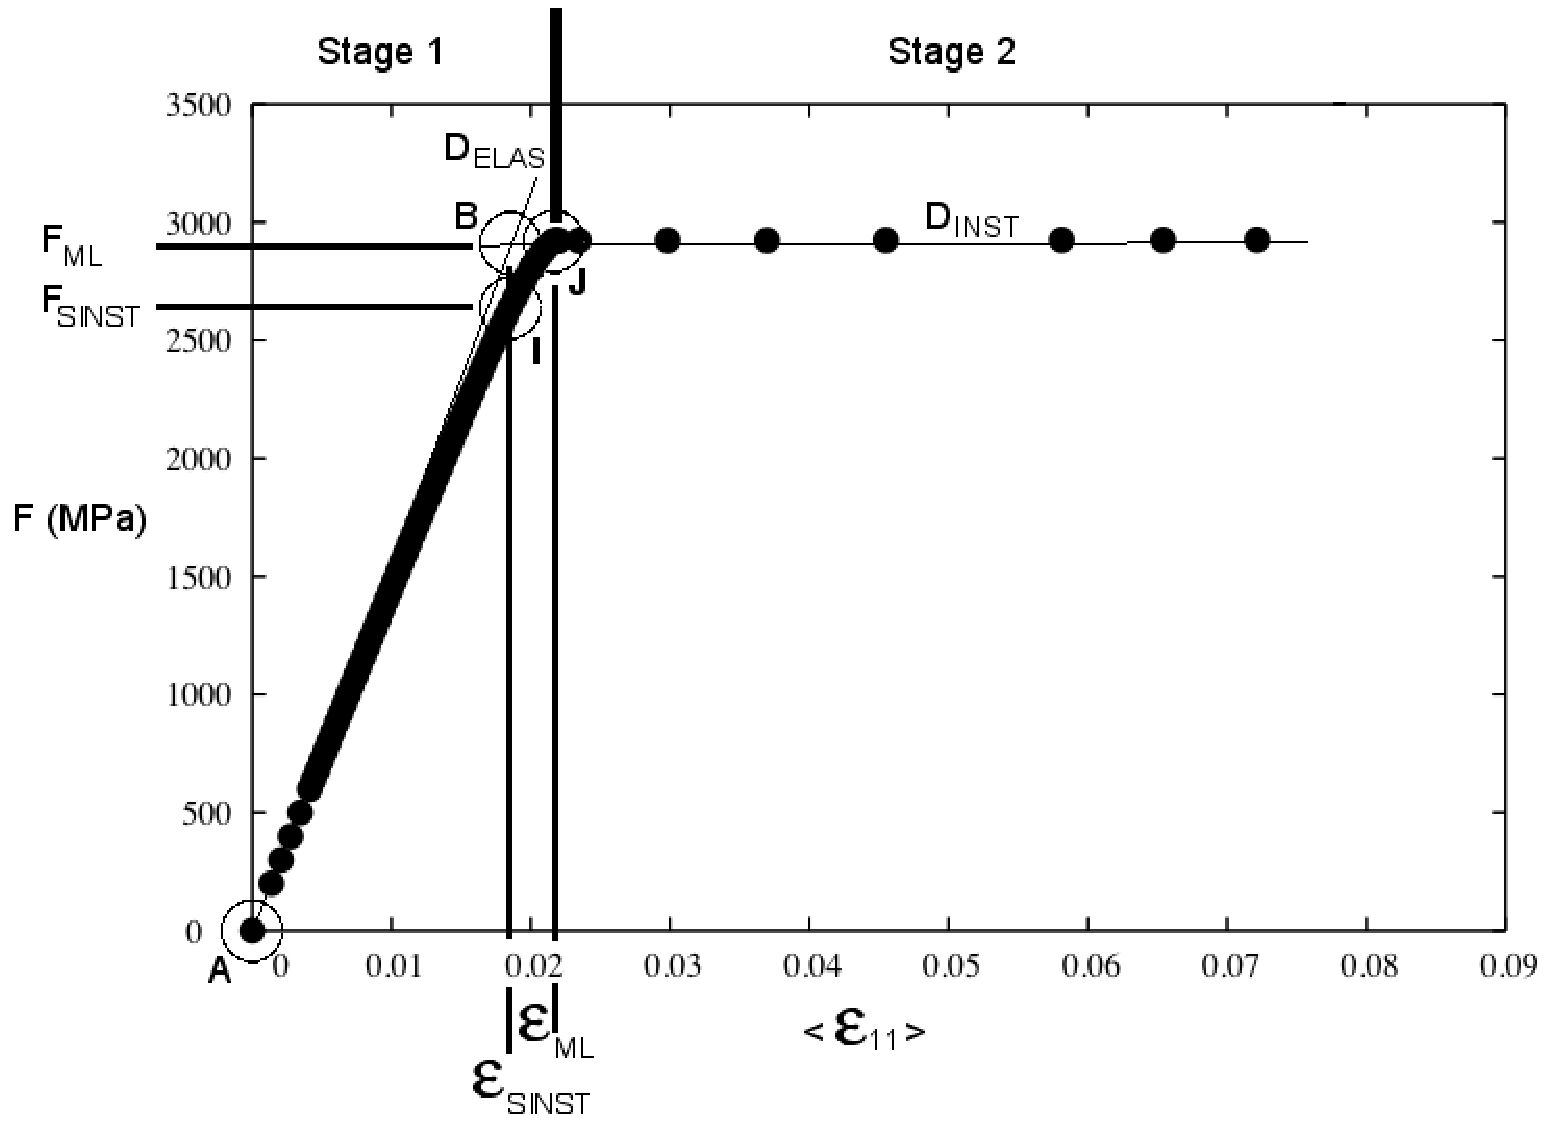
\includegraphics[scale=0.26]{chapters/chapter_model_mise_en_page/figures/figure_1.pdf} \\
		(a) \\
		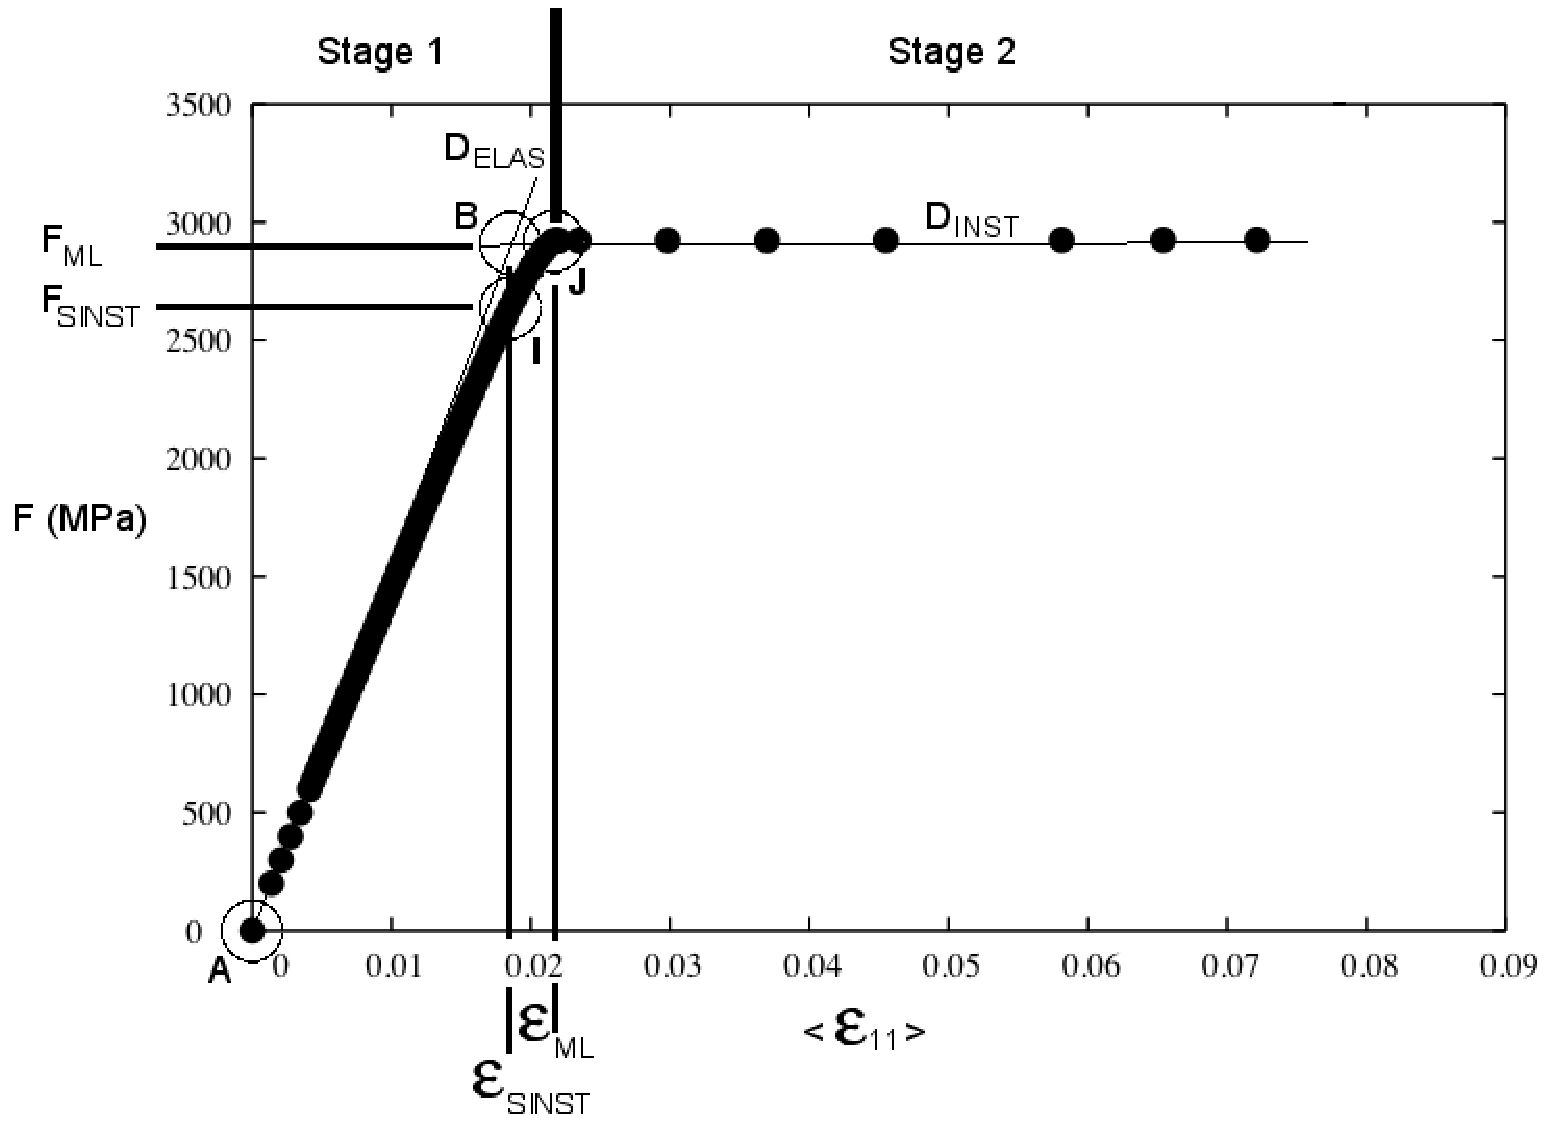
\includegraphics[scale=0.26]{chapters/chapter_model_mise_en_page/figures/figure_1.pdf} \\
		(b)
		\caption{
		\label{figure_chapter_xxx_lelabel}
			Typical loading curves. (a) xxx. (b) yyy.
		}
	\end{center}
\end{figure}

\section{Exemple de formule} \label{section_chapter_xxx_exemple_de_formule}


\begin{equation} \label{equation_chapter_xxx_lelabel}
\begin{split}
{C}^{loc}_{1111}({\cal{V}}(M),{\cal{D}}(M, t))& = V_{f}(M) C_{1111}^{f} (   1 - {\cal{D}}(M, t) )  \\
& + (1-V_{f}(M)) C_{1111}^{m}
\end{split}
\end{equation}





